Meine Beschäftigung mit Paul Otlet (1868-1944), dem großen belgischen
Privatgelehrten der \emph{Belle Époque}, ist jetzt genau zehn Jahre alt
und sie hat meine persönliche Auffassung von den Ursprüngen der
Informationsgesellschaft nachhaltig verändert. 2005 war ich von Boyd W.
Rayward, seinem Biographen, zu einem Symposium an die \emph{University
of Illinois at Urbana-Champaign} eingeladen worden, um über die
Zusammenarbeit von Otlet mit Otto Neurath aus Wien zu diskutieren,
dessen Projekt einer Wissensvisualisierung wiederum eines meiner
medienhistorischen Forschungsthemen ist.\footnote{Daraus entstand eine
  Art akademischer \emph{Social Graph} mit sehr fruchtbarem Output, der
  allein Boyd Raywards Verdienst als Organisator und Herausgeber zweier
  Bände ist: \emph{European Modernism and the Information Society:
  Informing the Present, Understanding the Past}, Farnham, Surrey:
  Ashgate 2008; \emph{Information Beyond Borders: International Cultural
  and Intellectual Exchange in the Belle Epoque}, Farnham, Surrey:
  Ashgate 2014.}

Es gab damals keine einzige deutschsprachige Publikation zu Paul Otlet,
und von seinem \emph{Traité de Documentation}\footnote{Paul Otlet:
  \emph{Traité de Documentation. Le livre sur le livre. Théorie et
  pratique}, Brüssel 1934 (Nachdruck 1989), online:
  \url{https://archive.org/details/OtletTraitDocumentationUgent}.}
existierten kaum Exemplare an deutschen Bibliotheken. Wo immer
Bibliotheken, Archive, Zettelkästen diskutiert worden sind, von
renommierten Autoren wie Umberto Eco, Dietrich Kerlen, Uwe Jochum bis
hin zu Markus Krajewksi --- überall blieb Paul Otlet eine Leerstelle in
den Darstellungen und Forschungsansätzen. Wir haben es mit einem Bruch
zu tun, der wie so vieles in der jüngeren europäischen Geistesgeschichte
auf die intellektuellen Verdrängungsereignisse des 2. Weltkrieges
zurückzuführen ist, aber auch auf die spätere Ignoranz gegenüber den
europäischen Beiträgen und Quellen zu den neuen
Informationstechnologien. Zwar erfolgte 1989 ein Nachdruck von Otlets
Hauptwerk, aber sein Projekt einer umfassenden Dokumentation in der
Universellen Bibliothek -- dem \emph{Mundaneum} -- blieb weitgehend
unbekannt.

Diese Leerstelle existierte nicht nur bei schlecht informierten
Medienwissenschaftlern, wo gern historisch uniformiert über Dinge
schwadroniert wird, die man lediglich aus anderen Publikationen kennt
und nicht aus der Archivforschung. Deutlich ist auch die Mythenbildung
der technischen Erfindungen, die alles in genuin amerikanische
Erfolgsgeschichten verlagert, was an Errungenschaften zu verzeichnen
wäre, vor allem im Hinblick auf das Internet und seine Anwendungen, auf
Dokumentverknüpfung und Metadaten. Die spannende Verbindung zu den
europäischen Ingenieuren\footnote{Beispielsweise von Emanuel Goldberg zu
  Vannevar Bush und seiner \emph{Memex} --- Vgl. dazu Michael Buckland:
  \emph{Vom Mikrofilm zur Wissensmaschine. Emanuel Goldberg zwischen
  Medientechnik und Politik}, Berlin: Avinus 2011. Zum europäischen
  Beitrag der Vernetzung und des WWW vgl. James Gillies, Robert Caillau:
  \emph{How The Web Was Born: The Story of the World Wide Web}, Oxford
  Univ. Press 2000.} und Intellektuellen, die dazu mehr als bloß
Grundlagen erarbeiteten, blieb einfach unbeachtet.

Was so verwunderlich nun auch wieder nicht ist: Nach der Publikation
seines Hauptwerkes im Jahr 1934 blieb das \emph{Mundaneum} in Brüssel
eine verschüttete Ruine und Paul Otlet eine weitgehend vergessene Figur,
bis 1968 der australische Wissenschaftler W. Boyd Rayward die
verlassenen Archivbestände zu erforschen begann, eine intellektuelle
Biographie Paul Otlets publizierte und später auch die englische
Übersetzung einer Auswahl seiner Essays besorgte.\footnote{W. Boyd
  Rayward: \emph{The Universe of Information. The Work of Paul Otlet for
  Documentation and International Organisation}, Moskau 1975 (FID 520).
  Boyd Rayward (ed.): \emph{International Organisation and Dissemination
  of Knowledge. Selected Essays of Paul Otlet}, Amsterdam, New York 1990
  (FID 684).} Aber erst das Zeitalter des World Wide Web regte die
Auseinandersetzung mit diesem Ausnahme-Intellektuellen wieder neu an,
namentlich war es der amerikanische Journalist Alex Wright, der in der
New York Times von einem ‚Ahnvater des Internet` zu berichten wusste,
ein Artikel, der mehr als einmal vom \enquote{Spiegel} mit ziemlich
irreführenden Titeln -- nun ja: übernommen wurde.\footnote{Vgl.
  \enquote{Internet: Vater der Zettelsuchmaschine}, Der Spiegel, 23.
  Juni 2008, und \enquote{Netzvisionär: Googles genialer Urahn}, Der
  Spiegel, 20. Juli 2011. Inzwischen erschien von Alex Wright:
  \emph{Cataloging the World. Paul Otlet and the Birth of the
  Information Age,} Oxford Univ. Press 2014.} Auf Otlet zurückgreifen
muss jedenfalls, wer diese Lücke im Verständnis der
Informationstechnologien schließen möchte.\footnote{Frank Hartmann
  (Hg.): \emph{Vom Buch zur Datenbank. Paul Otlets Utopie der
  Wissensvisualisierung}, Berlin 2012.}

Irreführend sagte ich deshalb, weil Otlet mangels Digitaltechnologie
weder ein World Wide Web der Dokumentenverknüpfung visioniert, noch eine
Suchmaschine im Stil von Google gebaut hat; er blieb an den Datenträger
Papier gebunden, wie heute die traurigen Relikte seiner Einrichtung
zeigen, die sich im belgischen Mons befinden.\footnote{Musée Mundaneum,
  Rue de Nimy 76, 7000 Mons, Belgien --- \url{http://www.mundaneum.org}.}
Seine Leistung hingegen war, wie schon bei Rayward nachzulesen steht,
die Organisation von Wissen durch dessen Klassifikation, teils im
Gegensatz, und teils in Überbietung des bibliothekarischen Prinzips
durch konsequente Weiterentwicklung von Metadaten. Ein bloßer Visionär
war er schon deshalb nicht, weil er eine abfrageorientierte
Wissensdatenbank tatsächlich eingerichtet und kostenpflichtig betrieben
hat; ab 1910 im Brüsseler \emph{Palais du Cinquantenaire}. Otlet hat
seine Ideen also durchaus realisiert und nicht nur visioniert. Dennoch
bereitete die damalige Technologie -- etwa von ihm entworfene
mechanische \emph{Meubles classeurs} -- große Schwierigkeiten
hinsichtlich der Funktionalität. Otlet stand mit all seinen
Schwierigkeiten eher am Ende des Gutenberg-Zeitalters als am Anfang der
Internet-Technologie. Deutlich erkennbar ist hingegen die Bewegung vom
monographischen Prinzip des Buches hin zur mobilen Wissensorganisation
der Datenbank.

\begin{figure}[htbp]
\centering
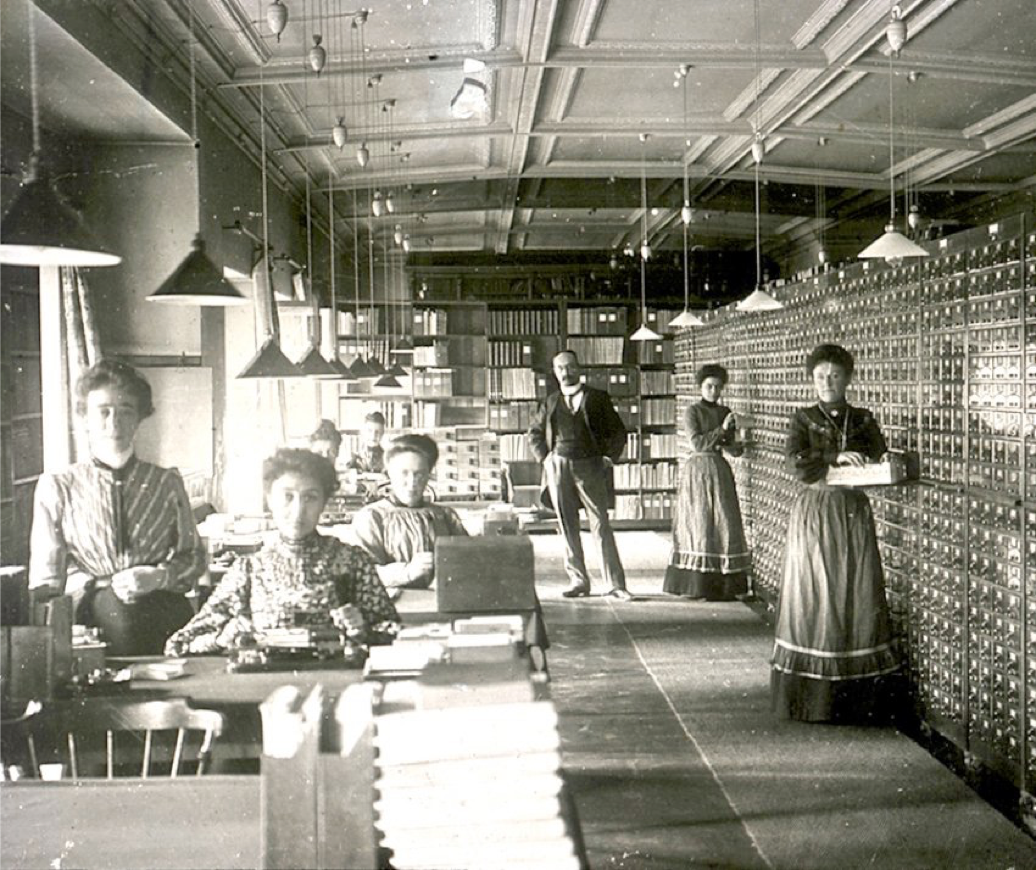
\includegraphics{img/Mundaneum1.png}
\caption*{Mitarbeiterinnen bei der Dokumentationsarbeit im Mundaneum,
Brüssel, ca. 1910 - Quelle (c) Mundaneum Mons, Belgien.}
\end{figure}

Da dem belgischen Privatier die Ordnung der Gutenberg-Galaxis nicht
länger angemessen schien, um im anbrechenden 20. Jahrhundert das
relevante Wissen zu repräsentieren, wandte er seine gesamte
intellektuelle Energie dafür auf, die \emph{Dokumentation} von
Information und Wissen neu zu strukturieren. Das ist ein postmoderner
Gedanke. Angesichts vielfältiger Problemlagen der beginnenden
Globalisierung musste ein neues Paradigma jenseits des Prinzips der
Monographie her, und für Otlet war das \emph{avant le mot} die
\enquote{Logik der Datenbank}.\footnote{Frank Hartmann: \enquote{Paul
  Otlet and the Logic of the Database}, in: Ars Electronica: \emph{Total
  Recall. The Evolution of Memory}, Ostfildern: Hatje Cantz 2013, S.
  38-45.} Er war letztlich ein Verfechter des Abschieds aus der Welt des
Datenträgers Papier und seiner Organisation in der Bibliothek, konnte
aber trotz technischer Ausführungen zum Mikrofilm nicht verdeutlichen,
dass Datenträger und Inhalte bis dato einer nahezu unbezwingbaren
kulturellen Logik der \enquote{weißen Magie}\footnote{Lothar Müller:
  \emph{Weiße Magie. Die Epoche des Papiers}, München 2012.} gehorchen,
die erst mit Magnetspeichern und Digitalmedien aufgelöst werden konnte.

\begin{figure}[htbp]
\centering
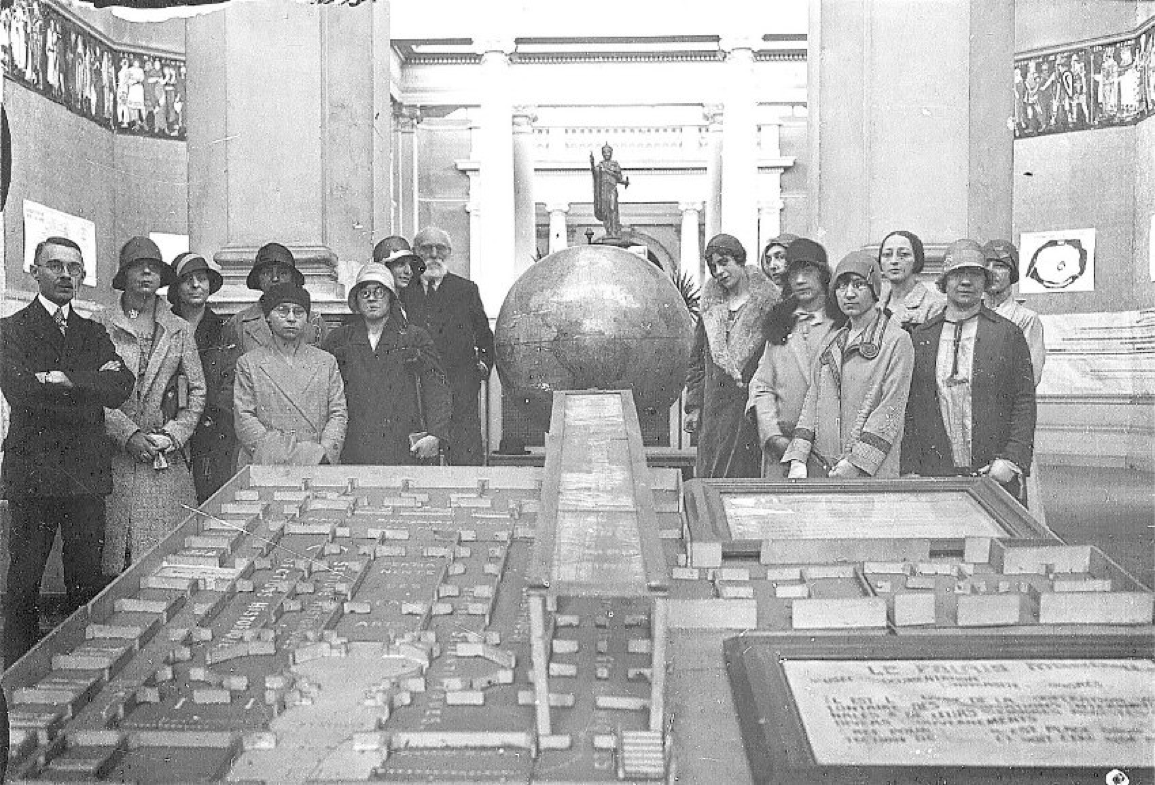
\includegraphics{img/Mundaneum2.png}
\caption*{Paul Otlet und Mitarbeiterinnen mit einem Modell der Weltstadt
des Wissens (im Palais de Cinquentanaire, Brüssl, ca. 1910) - Quelle (c)
Mundaneum Mons, Belgien.}
\end{figure}

Im Vorgriff auf eine Medienmoderne jedoch, dem später von McLuhan so
genannten \emph{Global Village}, erkannte Otlet die Chance, jene
Probleme zu lösen, die sich mit der Proliferation gedruckter
Publikationen ergaben: Man würde methodisch, technisch und
institutionell darauf reagieren müssen. In allen drei Bereichen leistete
er Grundlegendes, vor allem die Einrichtung der Ebene von Metadaten in
Form von Karteikarten sowie deren systematische Verwaltung. Darüber
hinaus sollte eine Weltstadt des Wissens, ein \emph{Mundaneum}, als
Zentrum in Genf, Rom oder Brüssel angesiedelt werden. So begriff Otlet
das Ende des bürgerlichen Buchzeitalters im Geiste der zentralen
Datenbank oder eines \emph{universellen} Buches, während die
Allgemeinheit noch in den Kategorien von Nationalmuseen und
Nationalbibliotheken dachte.

Bücher und Bibliotheken als Wissensspeicher fanden schon im ausgehenden
19. Jahrhundert ihre Kritiker. Schuld daran war wohl die explodierende
Produktion von Druckwerken aufgrund der umfassenden Industrialisierung.
Innovationen im Druckgewerbe hin oder her, es gab zudem die Nutzung der
Elektrizität für die Telekommunikation (Telegrafie) sowie neue
Aufzeichnungsverfahren (Fotografie, Phonographie) und Speichermedien wie
dem Mikrofilm, über dessen Einsatz zur Wissensorganisation Otlet wie
schon erwähnt einen Traktat verfasst hat.\footnote{Paul Otlet, Robert
  Goldschmidt: \emph{Livre Microphotographique. Le bibliophote ou livre
  à projection} (1910) in Hartmann (Hg.) 2012, S.159-168.}

\begin{figure}[htbp]
\centering
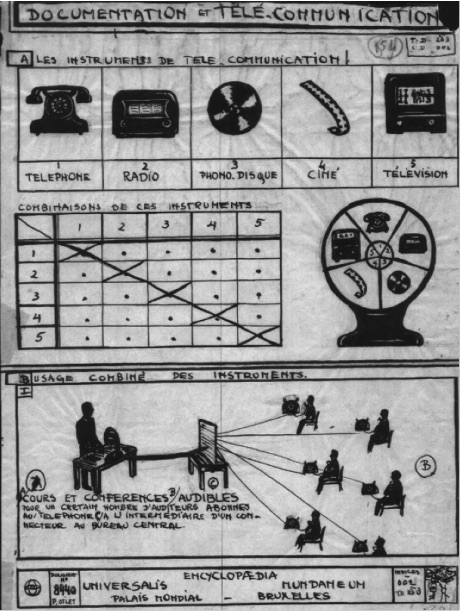
\includegraphics{img/Mundaneum3.jpg}
\caption*{Paul Otlets Skizze des \enquote{Hypermediums}: Dokumentation
und Telekommunikation, aus der Sammlung Encyclopedia Universalis, ca.
1934 - Quelle (c) Mundaneum Mons, Belgien.}
\end{figure}

Doch weniger die Möglichkeiten der Technik zur Handhabung von
Wissensbeständen, als die Klärung ihrer Logik wurde zu seinem
Lebenswerk: von der Überarbeitung von Deweys Dezimalklassifikation für
Bibliotheksbestände zur \emph{Classification décimale universelle} über
die Professionalisierung des Dokumentationswesen mittels Karteikarten
und Mikrofilm im \emph{Mundaneum} bis hin zum technisch noch
unausgereiften Entwurf eines globalen Wissens- und
Kommunikationsnetzes.\footnote{\enquote{Réseau de communication, de
  coopération et d'echanges à l'intervention d'un Centre Mondial}, Paul
  Otlet: Traité de Documentation. Le livre sur le livre. Théorie et
  pratique, Brüssel 1934, hier S.420.} Auf diesen Weg gebracht haben
ihn, meiner Ansicht nach, vor allem die seit 1851 regelmäßig
organisierten Weltausstellungen, deren Verstetigung im Sinne mancher
Zeitgenossen war -- die begehbare Welt-Enzyklopädie als ein integratives
Medium des gesamten Wissensbestandes. Vergessen wir hierbei nicht, dass
das Museum als künstliche Gedächtnismaschine eine ähnlich moderne Idee
der Repräsentation bürgerlichen Selbstbewusstseins ist, wie das auch für
die moderne Bibliothek als solche gilt. Sie geht zurück auf die
aufklärerische Forderung nach allgemeiner Publizität, eine politische
Maxime, die kein Geringerer als der deutsche Philosoph Immanuel Kant
1795 erhoben hat.\footnote{\enquote{Zum ewigen Frieden}, in: Immanuel
  Kant, Werkausgabe Band XI, hg. von Wilhelm Weischedel, Frankfurt am
  Main 1968, hier S. 244f.}

Ein Jahrhundert später gründete Otlet mit Henri La Fontaine das
\emph{Office International de Bibliographie} (1895) und begann mit dem
ambitionierten Projekt einer Indizierung aller möglichen
\enquote{Fakten} aus und über Publikationen mittels eines ausgeklügelten
Karteikartensystems, dem \emph{Répertoire Bibliographique Universel}.
Dies sollte ein Aufbewahrungsort des gesamten bekannten Bestandes an
Publikationen werden, an dem bereits die Absicht erkennbar wird, das
Buchformat beziehungsweise das monographische Prinzip zugunsten einer
flexiblen Wissensordnung aufzulösen, zu der neben Druckwerken auch Bild-
und Tondokumente gehören. Dieses Projekt besetzte jene technologische
Leerstelle, die eine im 19. Jahrhundert beginnende, die typografische
Epoche der Gutenberg-Galaxis\footnote{Marshall McLuhan: \emph{The
  Gutenberg Galaxy. The Making of Typographic Man}, Toronto 1962.}
aufsprengende neue Wissenskultur produziert hat.

Otlets Idee führt über den Anspruch einer bloßen Repräsentation von
Wissen in Bibliotheksbeständen deutlich hinaus. Seine Bewegung von
Museen und Bibliotheken hin zur umfassenden Dokumentation in der
Datenbank macht medienphilosophisch gesehen einen kategorialen
Unterschied in der Funktionalität aus, denn sie bricht mit der
Vorstellung, es könne eine \emph{substanzielle} Ordnung des Wissens
geben. Wissen ist immer kontextuell abhängig und folgt diskursimmanenten
Zwängen. Zwar ist es für Menschen unausweichlich, ihr Wissen und damit
ihre Umgebung in eine Ordnung zwingen zu wollen, um sie handhabbar zu
machen, doch diese Ordnung folgt niemals einer gegebenen Logik, sondern
einer veränderlichen Konstruktion, weil diese selbst abhängig ist von
den Forderungen und technischen Potenzialen ihrer Zeit.

So selbstverständlich uns heute die Tatsache scheint, auf alle möglichen
Inhalte unabhängig von ihren Datenträgern zugreifen zu können, so
unerhört war damals allein schon die Idee, Fragen des Wissensmanagements
außerhalb der exklusiven Routinen einer Buch- und Bibliothekskultur
anzusiedeln. Im Abschnitt \enquote{Inventions a faire} seines
\emph{Traité de documentation} formulierte Otlet eine Art Pflichtenheft
für Ingenieure, wobei die Automatisierung der Informationsarbeit als
Desideratum vorgestellt wird: An die Stelle der Schreibfläche und des
Datenträgers Papier träte dann ein universell zugänglicher Datenraum,
der räumlich und zeitlich durchforscht werden kann, und die Arbeit am
Schreibtisch würde durch eine neuartige Apparatur (ein
\emph{Hypermedium}) ersetzt: \enquote{La machinerie qui réaliserait ces
{[}\ldots{}{]} desiderata serait un véritable \emph{cerveau mécanique et
collectif}.}\footnote{Otlet, \emph{Traité}, a.a.O., S.391.} In mehreren
detaillierten Punkten wird in erstaunlicher Weise die Reformation der
gesamten intellektuellen Arbeit angekündigt, als Vorstellung einer
telematischen Kulturtechnik einerseits, als Bruch mit der Verbindung von
Daten und Bedeutungen andererseits. Beides bezeichnet die Logik der
Datenbank: Wissensgenerierung unabhängig vom jeweiligen Ort und Kontext.
Doch dieses Problem wird nur benannt, und ist ja trotz aller Automaten
bis heute -- Stichwort: \emph{Semantic Web} -- nicht wirklich gelöst.
Seit Leibniz und wohl auch schon länger geht es darum, mechanische
Kunstgriffe zu entwickeln und diese zu automatisieren: Rechenapparate
nicht zum Ausdruck von Gedanken zu nutzen, sondern zur Delegierung von
Entscheidungen an das, was man heute nicht ganz zu Recht als
bedrohlich-befremdende Welt der Algorithmen wahrnimmt.\footnote{Zur
  weiteren Diskussion dieser Bedrohlichkeit vgl. Jaron Lanier: \emph{Wem
  gehört die Zukunft?} Hamburg 2014.}
